% ==============================================================================================================
\section{Orbital optimized \textit{q}-pUCCD}\label{sez:orbital-optimization}

In questa sezione viene illustrata l’implementazione di un circuito $q$-oo-pUCCD basato sull’ottimizzazione orbitale. Si parte dalla costruzione teorica dell’operatore di rotazione $\hat{\mathcal{K}}$ per modificare la base degli orbitali, adattando dinamicamente gli integrali dell'hamiltoniana per ogni iterazione del processo VQE. Questo approccio ottimizza direttamente la forma della funzione d’onda e permette di esplorare configurazioni che minimizzano l’energia dell’ansatz scelto. 

% --------------------------------------------------------------------------------------------------------------
\subsection{Costruzione del circuito \textit{q}-oo-pUCCD}\label{subsec:costruzione-oo-pUCCD}

Per implementare attraverso un circuito l'operatore $e^{\hat{\mathcal{K}}}$ si parte dal considerare le possibili rotazioni di coppie di orbitali di spin, cioè le entrate non nulle della matrice anti-hermitiana $\hat{\mathcal{K}}$ introdotta in Sezione~\ref{eqn:ansatz-oo-pUCCD}, qui sotto riportata:

\begin{equation*}
    \hat{\mathcal{K}} = \sum_{p<q} \mathcal{K}_{pq} (a_{q}^{\dagger}a_{p} - a_{p}^{\dagger}a_{q})
\end{equation*}

La funzione \myinline{create_orbital_rotation_list} genera la lista ordinata delle rotazioni tra orbitali con indici $p<q$, nella forma \myinline{[0,1]}, \myinline{[0,2]} e così via.

% orbital opt ___________________________________________________
\begin{tcolorbox}[title=Generazione lista di eccitazioni]
\begin{lstlisting}
def create_orbital_rotation_list(ansatz) -> list:

half_as = int(ansatz.num_qubits / 2)
orbital_rotations = []

for i in range(half_as):
        for j in range(half_as):
            if i < j:
                orbital_rotations.append([i, j])
                
return orbital_rotations
\end{lstlisting}
\vspace{-0.2cm}
\end{tcolorbox}

Successivamente, si converte ogni coppia di indici $(p,q)$ in un operatore fermionico $a^{\dagger}_{q} a_p$ con la funzione \myinline{build_fermionic_excitation_ops}
    
% orbital opt ___________________________________________________
\begin{tcolorbox}[title=Costruzione operatore fermionico, breakable]
\begin{lstlisting}
def build_fermionic_excitation_ops(
    mo_problem, 
    excitations: Sequence,
    mapper: QubitMapper = JordanWignerMapper()
    ) -> list[FermionicOp]:
    
    num_spin_orbitals = 2 * mo_problem.num_spatial_orbitals
    operators = []

    for exc in excitations:
        label = []
        for occ in exc[0]:
            label.append(f"+_{occ}")
        for unocc in exc[1]:
            label.append(f"-_{unocc}")
        op = FermionicOp({" ".join(label): 1}, num_spin_orbitals=num_spin_orbitals)
        op_adj = op.adjoint()
        # va considerata una fase immaginaria introdotta dalla approssimazione di 
        # Trotter implementata in Qiskit

        op_minus = 1j * (op - op_adj)
        operators.append(op_minus)
        
        # map to qubit operators
        qubit_ops = mapper.map(operators)

    return qubit_ops
\end{lstlisting}
\vspace{-0.2cm}
\end{tcolorbox}

Infine, si usa la classe \myinline{EvolvedOperatorAnsatz} per costruire il circuito con le eccitazioni esponenziate. Quest'ultimo va poi concatenato a $q$-pUCCD, passato in argomento come \myinline{initial_state}, per formare $q$-oo-pUCCD.

% orbital opt ___________________________________________________
\begin{tcolorbox}[title=Generazione ansatz oo-pUCCD, breakable]
\begin{lstlisting}
def generate_oo_puccd (puccd, mo_problem, excitations):

    qubit_ops = build_fermionic_excitation_ops(
        mo_problem, 
        excitations
        )

    oo_puccd = EvolvedOperatorAnsatz(
        operators=qubit_ops,
        initial_state=puccd,
        parameter_prefix='k'
    )

    bounds = [[-np.pi,np.pi] for _ in range(
             oo_puccd.num_parameters)]
    oo_puccd.parameter_bounds = bounds

    return oo_puccd
\end{lstlisting}
\vspace{-0.2cm}
\end{tcolorbox}


% --------------------------------------------------------------------------------------------------------------
\subsection{oo-VQE}\label{sez:oo-VQE}

L'operazione di ottimizzazione orbitale avviene in concomitanza con VQE, motivo per cui spesso ci si riferisce questo algoritmo con la sigla oo-VQE: durante la minimizzazione dell'energia si ricalcola l'hamiltoniana ad ogni ottimizzazione dei parametri. Per poterlo fare, bisogna accedere agli integrali a uno e due corpi, contenuti nell'attributo \myinline{hamiltonian} dell'\myinline{ElectronicStructureProblem} in forma di classe, un oggetto chiamato \myinline{ElectronicIntegrals}. Al suo interno, gli integrali sono divisi per spin, perciò occorrono due matrici: $\hat{\mathcal{K}}_\alpha$ e $\hat{\mathcal{K}}_\beta$, costruite sempre a partire dalla lista di eccitazioni \myinline{orbital_rotations}. 
La funzione \myinline{orbital_rotation_matrix} riceve in argomento i parametri restituiti da ciascuna interazione del ciclo VQE e li inserisce all'interno delle matrici $\hat{\mathcal{K}}$, quindi restituisce gli operatori di rotazione $e^{\hat{\mathcal{K}}_\alpha}$, $e^{\hat{\mathcal{K}}_\beta}$.

% orbital opt ___________________________________________________
\begin{tcolorbox}[title=Costruzione $e^{\hat{\mathcal{K}}}$, breakable]
\begin{lstlisting}
def orbital_rotation_matrix(
    problem, 
    parameters: np.ndarray, 
    rotations: list
    ) -> Tuple[np.ndarray, np.ndarray]:

    dim_kappa_matrix = problem.num_spatial_orbitals
    
    k_matrix_alpha = np.zeros((dim_kappa_matrix, dim_kappa_matrix))
    k_matrix_beta  = np.zeros((dim_kappa_matrix, dim_kappa_matrix))
    
    for i, exc in enumerate(rotations):
        k_matrix_alpha[exc[0]][exc[1]] =  parameters[i]
        k_matrix_alpha[exc[1]][exc[0]] = -parameters[i]
        k_matrix_beta[exc[0]][exc[1]]  =  parameters[i]
        k_matrix_beta[exc[1]][exc[0]]  = -parameters[i]

    matrix_a = expm(k_matrix_alpha)
    matrix_b = expm(k_matrix_beta)
    
    return matrix_a, matrix_b
\end{lstlisting}
\vspace{-0.2cm}
\end{tcolorbox}

Dopodiché si può procedere con la modifica degli integrali, utilizzando le relazioni \ref{eqn:trasformazione-integrali}. Queste vengono implementate utilizzando \myinline{numpy} per ottimizzare il calcolo il più possibile, dal momento che il numero di moltiplicazioni richieste scala come $\mathcal{O}(K^4)$, con $K$ numero di orbitali spaziali. 
In realtà, nello specifico del caso di $q$-pUCCD, \myinline{ElectronicIntegrals} contiene soltanto valori associati a spin $\alpha$, pertanto \myinline{matrix_b} può essere ignorata. 
Una volta effettuate le trasformazioni degli integrali, si può andare ad estrarre la nuova hamiltoniana di seconda quantizzazione (eq. \ref{eqn:hamiltoniana-seconda-q}) dal problema elettronico ruotato.

% orbital opt ___________________________________________________
\begin{tcolorbox}[title=Rotazioni orbitali, breakable]
\begin{lstlisting}
def rotate_orbitals(
    problem, 
    one_body, 
    two_body, 
    matrix_a, 
    matrix_b, 
    mapper = JordanWignerMapper()
    ): 

    C = matrix_a  # Matrice C = exp(K_a)

    N = len(C)

    # Trasformazione degli integrali a un corpo
    one_body_transformed = np.einsum('up,uv,vq->pq', C, one_body, C)
    # Trasformazione degli integrali a due corpi
    eri_transformed = np.einsum('up,vq,xr,ys,uvxy->pqrs', C, C, C, C, eri)
    eri_transformed = np.zeros((N, N, N, N))
    # Definizione di un oggetto ElectronicIntegrals per modificare quello contenuto in problem
    e_int = ElectronicIntegrals.from_raw_integrals(
        h_transformed,                                            
        eri_transformed
    )

    problem.hamiltonian.ElectronicIntegrals = e_int

    # extract rotated operator
    rotated_operator = problem.hamiltonian.second_q_op()
    rotated_operator = mapper.map(rotated_operator)

    return rotated_operator
\end{lstlisting}
\vspace{-0.2cm}
\end{tcolorbox}

Su questo \myinline{rotated_operator} sarà calcolato il valore di aspettazione (eq. \ref{eqn:energia-oo-pUCCD}) nel ciclo successivo di VQE, nel quale saranno ottimizzati ulteriormente i parametri, che poi saranno usati per generare una nuova matrice di rotazione; questo procedimento quindi continua fino a convergenza.

% --------------------------------------------------------------------------------------------------------------
\subsection{Risultati}\label{sez:risultati-oo-pUCCD}

In questa sezione si riportano i risultati ottenuti applicando l’ottimizzazione orbitale nella simulazione delle molecole LiH e H$_2$O, per osservare il comportamento di questo approccio su un sistema più complesso, evidenziando eventuali limiti e vantaggi scalabili a sistemi di dimensioni maggiori.

% ..............................................................................................................
\subsubsection{LiH}

Nel caso dell'idruro di litio, il circuito $q$-oo-pUCCD comporta un aumento in profondità di solamente 155, il che renderebbe questo ansatz estremamente promettente, se fosse anche capace di migliorare sensibilmente i risultati di pUCCD. In realtà, per quanto riguarda l'energia di stato fondamentale, è osservata una diminuzione del valore calcolato, ma non di certo degna di nota. Il valore di energia a grandi distanze invece giova della correzione, compatibilmente con quanto osservato in altri studi \cite{Sokolov_2020,Zhao_2023}, anche se non nella stessa misura.

\begin{figure}[H]
    \centering
    \hspace{-1cm}
    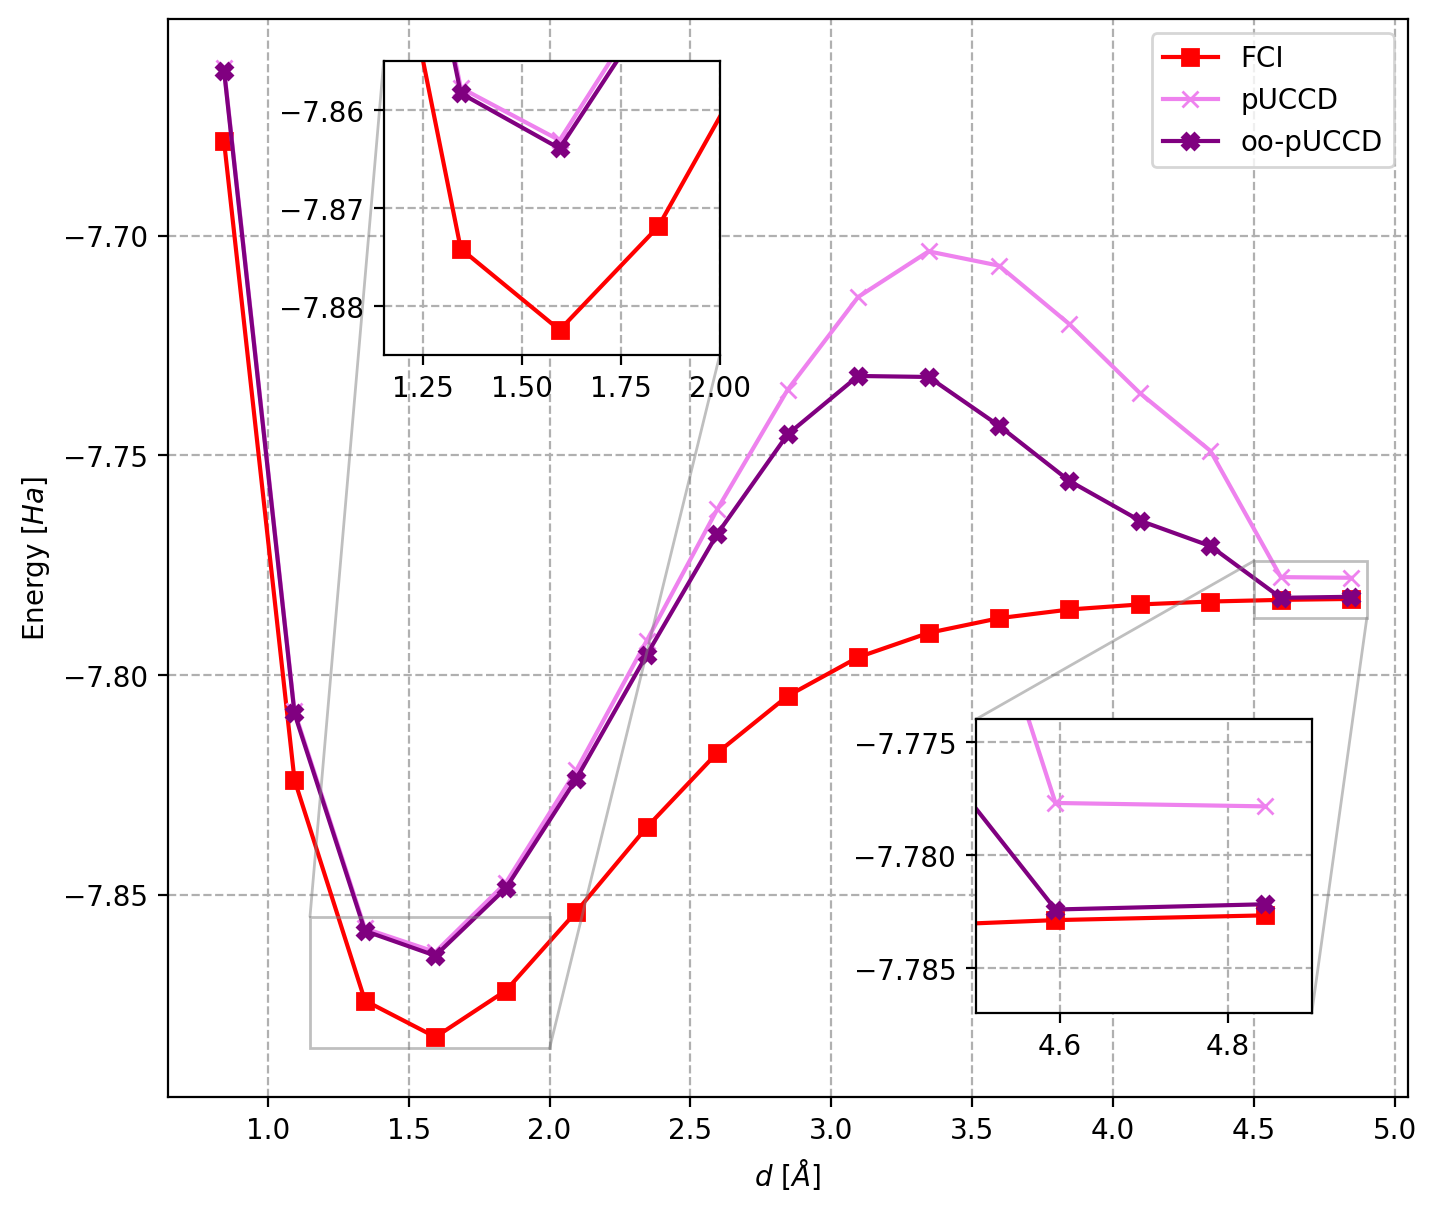
\includegraphics[width=.6\linewidth]{Immagini/Capitolo_3/LiH_oo_pUCCD.png}
    \caption{LiH: $q$-pUCCD con ottimizzazioni orbitali.}
    \label{fig:LiH-ottimizzazioni-orbitali}
\end{figure}

% Please add the following required packages to your document preamble:
% \usepackage[table,xcdraw]{xcolor}
% Beamer presentation requires \usepackage{colortbl} instead of \usepackage[table,xcdraw]{xcolor}
\begin{table}[H]
    \centering
    \begin{tabular}{|c|c|c|c|c|c|c|}
    \hline
    \textbf{Metodo}                                              & \textbf{Depth} & \textbf{CNOT} & \textbf{Parametri} & \textbf{$E_0$} & \textbf{$E_\infty$} & \textbf{$\Delta E_{\text{max}}$} \\ \hline
    \textbf{\color[HTML]{CB0000} FCI}       & /              & /             & /                  & -7.8824        & -7.7827             & /                                \\ \hline
    \textbf{\color[HTML]{D952D8} $q$-pUCCD} & 511            & 384           & 4                  & -7.8630        & -7.7779             & 0.09                             \\ \hline
    \textbf{\color[HTML]{6200C9} $q$-oo-pUCCD}               & 666           & 464           & 14                 & -7.8639        & -7.7822             & 0.06                             \\ \hline
\end{tabular}
\caption{Energie calcolate in hartree e dimensioni circuiti oo-LiH.}
\label{tab:oo-LiH}
\end{table}

La differenza nei minimi di energia tra $q$-pUCCD e $q$-oo-pUCCD è di appena $0.8$~mHa, come riportato nella Tabella~\ref{tab:oo-LiH}, mentre a grande distanza raggiunge i $15$~mHa, abbassando la deviazione dal valore di riferimento FCI a soltanto $0.5$~mHa.


% ..............................................................................................................
\subsubsection{H$_2$O}

Per testare ulteriormente le potenzialità dell'algoritmo oo-VQE, si applica ad un sistema più laborioso: la molecola di H$_2$O.
Anche in questo caso si utilizza \myinline{FreezeCoreTransformer} per ridurre la dimensione del problema, che stavolta porta all'esclusione di due orbitali \inglese{core}. La differenza in profondità tra i circuiti si fa più marcata rispetto a LiH, con $q$-oo-pUCCD che contiene oltre $250$ \inglese{layers} in più dei circa $1100$ di pUCCD. Tuttavia, si tratta ancora di un circuito piuttosto contenuto, soprattutto considerando che $q$-UCCSD per lo stesso problema supererebbe una profondità di $10000$.

\begin{figure}[H]
    \centering
    \hspace{-1cm}
    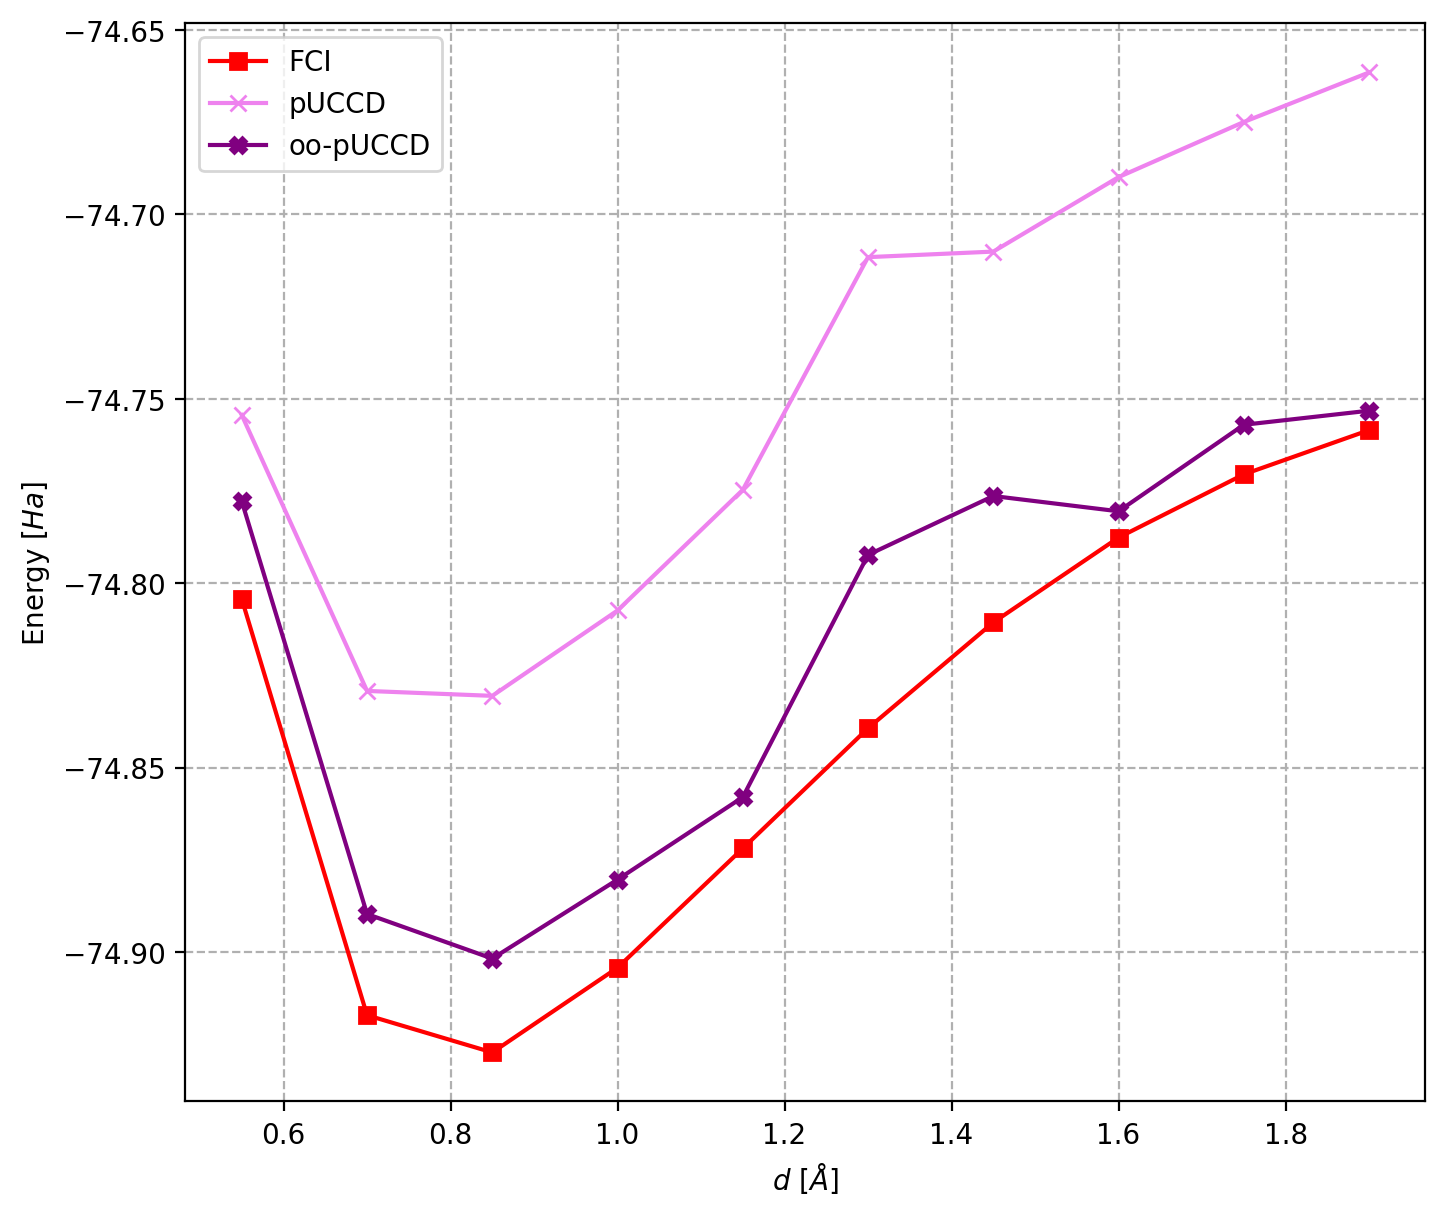
\includegraphics[width=.6\linewidth]{Immagini/Capitolo_3/H2O_oo_pUCCD.png}
    \caption{H$_2$O: $q$-pUCCD con ottimizzazioni orbitali.}
    \label{fig:H2O-ottimizzazioni-orbitali}
\end{figure}

% Please add the following required packages to your document preamble:
% \usepackage[table,xcdraw]{xcolor}
% Beamer presentation requires \usepackage{colortbl} instead of \usepackage[table,xcdraw]{xcolor}
\begin{table}[H]
    \centering
    \begin{tabular}{|c|c|c|c|c|c|}
    \hline
    \textbf{Metodo} & \textbf{Depth} & \textbf{CNOT} & \textbf{Parametri} & \textbf{$E_0$} & \textbf{$\Delta E_{\text{max}}$} \\ \hline
    \textbf{\color[HTML]{CB0000} FCI}           & /      & /      & /     & -74.927   & /       \\ \hline
    \textbf{\color[HTML]{D952D8} $q$-pUCCD}     & 1145   & 896    & 8     & -74.831   & 0.13    \\ \hline
    \textbf{\color[HTML]{6200C9} $q$-oo-pUCCD}  & 1396   & 1036   & 23    & -74.902   & 0.05    \\ \hline
\end{tabular}
\caption{Energie calcolate in hartree e dimensioni circuiti oo-H$_2$O.}
\label{tab:oo-H2O}
\end{table}

In questo caso, osservando la Figura~\ref{fig:H2O-ottimizzazioni-orbitali} e la Tabella~\ref{tab:oo-H2O}, il vantaggio offerto dalle ottimizzazioni orbitali nel calcolo dell'energia è lampante: il minimo diminuisce di oltre $70$~mHa, il valore a grandi distanze scende fino a discostarsi di soli $5$~mHa dal valore FCI. Oltre a questo, l’ottimizzazione orbitale permette di recuperare una frazione significativa del valore assoluto corretto dell’energia totale a tutte le geometrie studiate, mantenendo una precisione entro $10$~mHa rispetto ai calcoli di riferimento e riproducendo, almeno qualitativamente, i profili energetici corretti.

Riassumendo, questi risultati suggeriscono l'ansatz $q$-oo-pUCCD può offrire un sensibile miglioramento nella precisione energetica, particolarmente significativo nelle energie a lungo raggio. Allo stesso tempo, l’incremento di profondità si mantiene limitato, soprattutto in confronto agli ansatz UCC più strutturati. In particolare, nel caso di H$_2$O, si osserva un miglioramento sostanziale sia a grandi distanze che nella zona del minimo, rendendo il metodo interessante per applicazioni future, nelle quali potrebbe costituire un approccio bilanciato fra una buona approssimazione energetica e una complessità circuitale contenuta.